\section{Reidemeister 1, 2  rewrites}


We strengthen our formalism by the introduction of the Reidemeister 1 (Definition \ref{r1}) and Reidemeister 2 (Definition \ref{r2}) rewrites. We shall use the sign "$\displaystyle \longleftrightarrow$" for a rewrite, but also for any finite sequence of pattern matchings and rewrites. 

\begin{definition}
For any node variable $a \in \Upsilon$: 
\begin{enumerate}
\item[-] the first R1 rewrite is: $\displaystyle a^{x} x \, \longleftrightarrow \, x$
\item[-] the second R1 rewrite is:  $\displaystyle \bar{a}^{x} x \, \longleftrightarrow \, x$
\end{enumerate}
\centerline{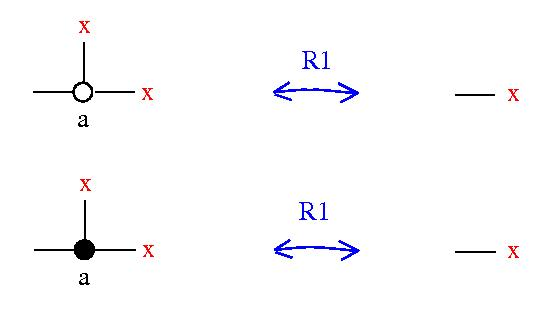
\includegraphics[width=80mm]{jpg/r1.jpg}}  
\label{r1}
\end{definition}



\begin{definition}
For any node variable $a \in \Upsilon$: 
\begin{enumerate}
\item[-] the first R2 rewrite is: $\displaystyle \left(\bar{a} a \right)^{e} x \, \longleftrightarrow \, x$
\item[-] the second R2 rewrite is:  $\displaystyle \left(a  \bar{a}\right)^{e} x \, \longleftrightarrow \, x$
\end{enumerate}
\centerline{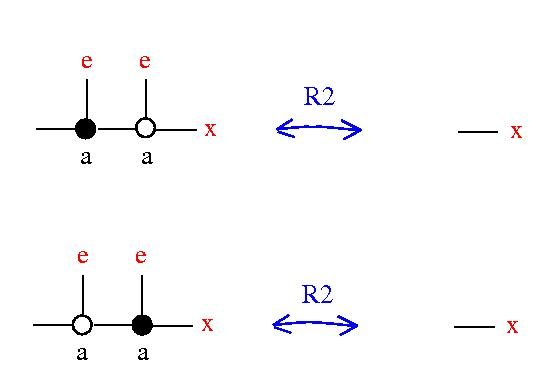
\includegraphics[width=80mm]{jpg/r2.jpg}}
\label{r2}
\end{definition}





\begin{proposition}
The first R1 rewrite is equivalent with the enforcing of the equation (\ref{a0}), in the sense that for any $a \in \Upsilon$ 
\begin{equation}
 (a 0)^{e} x \, \longleftrightarrow 0^{e} x 
\label{a01r1}
\end{equation}

The second R1 rewrite is equivalent with the first R1 rewrite and:  for any $a \in \Upsilon$ 
\begin{equation}
 ((a-1) 0)^{e} x \, \longleftrightarrow 0^{e} x 
\label{a02r1}
\end{equation}
\end{proposition}

 
\paragraph{Proof.} For the first R1 rewrite part the proof is  in the Figure \ref{a0r1-fig}. (This is almost similar with Figure \ref{a0-fig})
\begin{figure}[h]\centerline{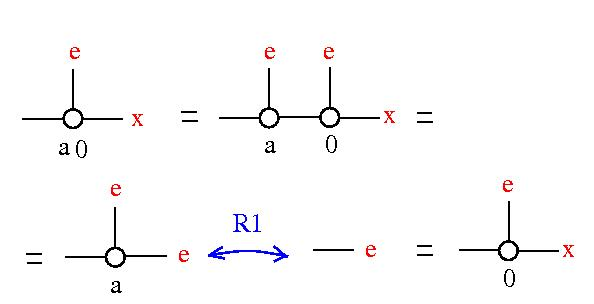
\includegraphics[width=80mm]{jpg/a0r1.jpg}}  \caption{ The first R1 rewrite is equivalent with $a 0 = 0$ } \label{a0r1-fig} \end{figure}
For the second R1 rewrite part see  the Figure \ref{a-1r1-fig}. 
\begin{figure}[h]\centerline{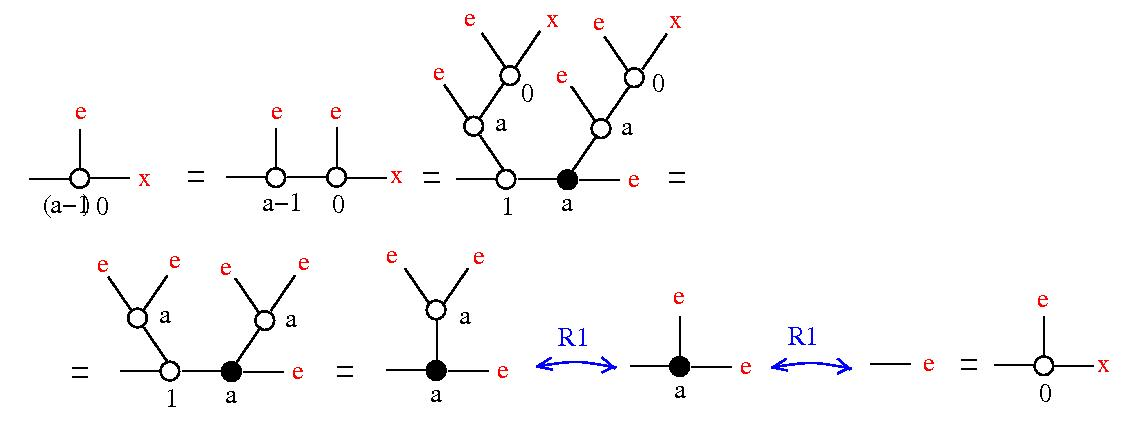
\includegraphics[width=120mm]{jpg/a-1r1.jpg}}  \caption{ The second R1 rewrite is equivalent with $(a-1) 0 = 0$ } \label{a-1r1-fig} \end{figure}

\vspace{.5cm}


The Reidemester 2 rewrites are related to pattern matching equalities (\ref{a-a}) and (\ref{a-(a-b)}),  from the Figures \ref{a-a-fig} and \ref{a-(a-b)-fig}.  

\begin{proposition}
The second R2 rewrite implies that for any $a \in \Upsilon$
\begin{equation} 
 (a - (a - 0))^{e} x \, \longleftrightarrow 0^{e} x 
\label{2r2}
\end{equation}
Conversely, (\ref{2r2}) implies that the first R2 rewrite is equivalent with: for any $a \in \Upsilon$
\begin{equation} 
 (a - (a - 1))^{e} x \, \longleftrightarrow 0^{e} x 
\label{1r2}
\end{equation}
\label{pr2}
\end{proposition}





\paragraph{Proof.} For the first implication see the Figure \ref{a-a-0r2-fig}. For the second implication see the Figure \ref{a-a-1r2-fig}. 
\begin{figure}[h]\centerline{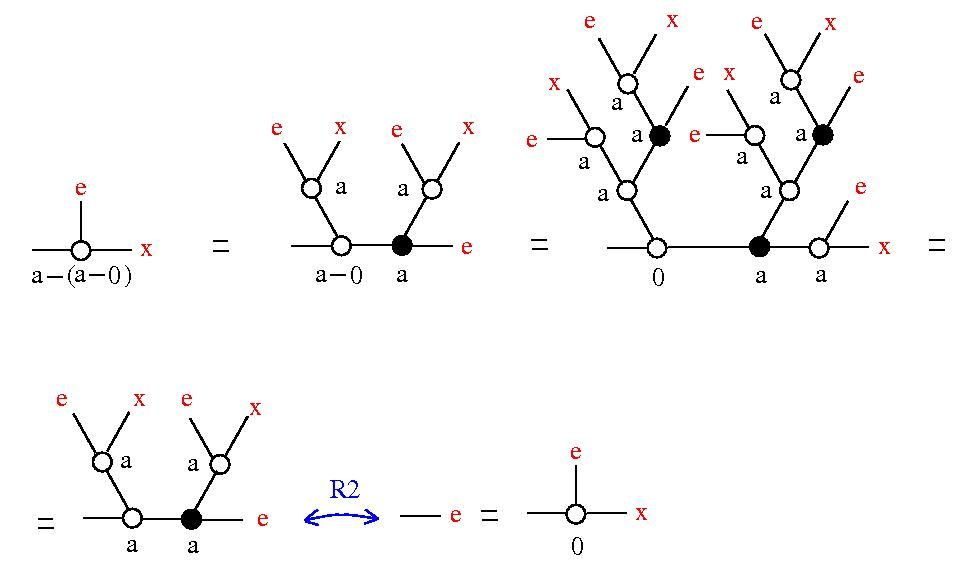
\includegraphics[width=120mm]{jpg/a-a-0r2.jpg}}  \caption{ The second R2 rewrite implies $a-(a-0) = 0$ } \label{a-a-0r2-fig} \end{figure}

\begin{figure}[h]\centerline{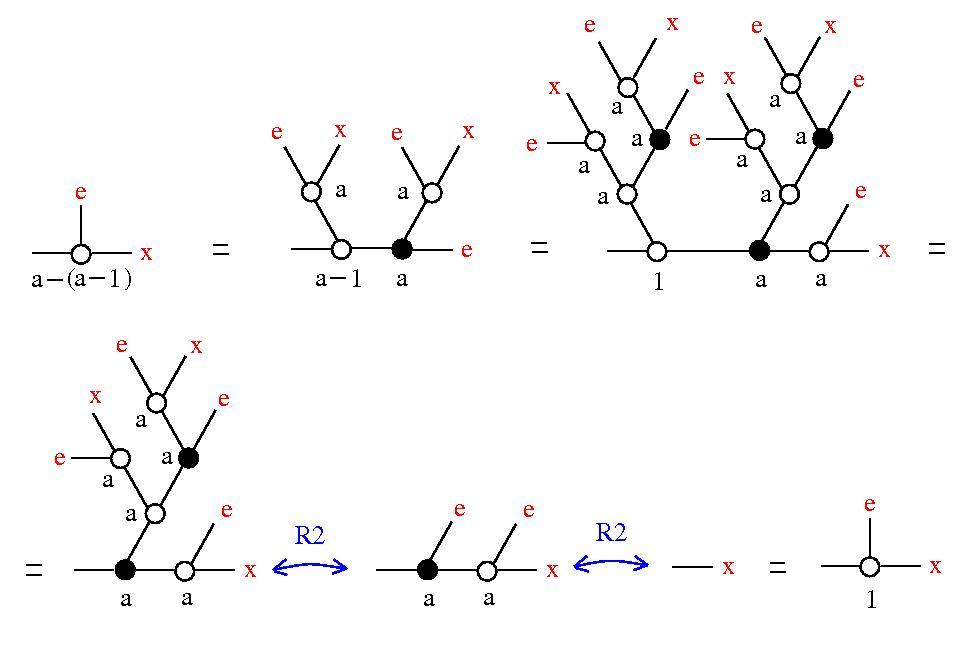
\includegraphics[width=120mm]{jpg/a-a-1r2.jpg}}  \caption{ The first R2 rewrite is equivalent with $a-(a-1) = 1$ } \label{a-a-1r2-fig} \end{figure}

\vspace{.5cm}

